% MQTT vs LwM2M Playground - design, architecture and workflow
% Compile with:  pdflatex playground.tex   (run twice for the table of contents)
% Uses only standard packages (TeX Live / MiKTeX / Overleaf).

\documentclass[11pt,a4paper]{article}

\usepackage[T1]{fontenc}
\usepackage[utf8]{inputenc}
\usepackage{lmodern}
\usepackage[margin=2.3cm]{geometry}
\usepackage{xcolor}
\usepackage{booktabs}
\usepackage{tabularx}
\usepackage{longtable}
\usepackage{enumitem}
\usepackage{listings}
\usepackage{tikz}
\usetikzlibrary{arrows.meta,positioning,fit,calc,shapes.geometric}
\usepackage[hidelinks]{hyperref}
\usepackage{caption}

\definecolor{mqtt}{HTML}{2A78D6}
\definecolor{lwm2m}{HTML}{EB6834}
\definecolor{ota}{HTML}{1BAF7A}
\definecolor{boxfill}{HTML}{F2F1ED}
\definecolor{codebg}{HTML}{F6F6F3}

\lstset{
  basicstyle=\ttfamily\small,
  backgroundcolor=\color{codebg},
  frame=single,
  rulecolor=\color{black!15},
  breaklines=true,
  columns=fullflexible,
  keepspaces=true,
  showstringspaces=false,
  xleftmargin=2pt,
  xrightmargin=2pt
}

\newcommand{\code}[1]{\texttt{#1}}
\setlist{itemsep=2pt,topsep=4pt}

\title{\textbf{MQTT vs LwM2M Playground}\\[4pt]
\large An embedded-C IoT protocol laboratory on a PC\\
Design, architecture, workflow and measurement approach}
\author{Phase 1 -- simulated devices, real servers}
\date{October 2026}

\begin{document}
\maketitle

\begin{abstract}
This document describes a software laboratory for learning and benchmarking
two IoT device-management and telemetry protocols, MQTT and LwM2M, before any
hardware is available. Simulated sensor devices are written in C with the same
libraries an STM32 would use (Eclipse Paho MQTTPacket, Eclipse Wakaama,
mbedTLS) and talk to real servers (Eclipse Mosquitto and Eclipse Leshan). A
small C web server (the \emph{lab}) starts the devices, observes both servers
and streams every protocol message to an interactive browser dashboard. The
document covers the goals and constraints, the architecture, every component,
the end-to-end workflow, how measurements are taken, the network and security
experiments, the simulated OTA exercise, how the system was verified, the
problems found during development and how they were fixed, measured results,
known limitations, and the plan for porting to STM32 + Quectel EC200U.
\end{abstract}

\tableofcontents
\newpage

%======================================================================
\section{Goals and constraints}

\subsection{What the laboratory is for}
\begin{itemize}
  \item Learn MQTT and LwM2M \emph{by interacting with them}: see every
        message (\code{CONNECT}, \code{PUBLISH}, \code{REGISTER},
        \code{NOTIFY}, ...), its bytes and its timing.
  \item Compare the two protocols with honest measurements: latency, bytes on
        the wire, connection cost, success rate.
  \item Experiment with bad networks (latency, packet loss) and with security
        (TLS, DTLS) and see the effect immediately.
  \item Produce code that can later be moved to an STM32 with an EC200U
        cellular modem without rewriting the protocol logic.
\end{itemize}

\subsection{Constraints that shaped the design}
\begin{itemize}
  \item \textbf{No hardware.} Everything runs on a Windows PC; Linux/macOS/WSL
        must work too.
  \item \textbf{Devices in C, no Python.} The simulated devices must be
        embedded-style C so the code is portable to a microcontroller. Python
        must not be required to run anything.
  \item \textbf{Real servers.} Mosquitto and Leshan, not mocks.
  \item \textbf{No fabricated numbers.} A value that was not measured is shown
        as ``Not measured''; a failed message has no latency.
  \item \textbf{Small and playable first.} Milestones in order: MQTT sample,
        LwM2M sample, dashboard, benchmark, security, network simulation, OTA.
\end{itemize}

%======================================================================
\section{Overall architecture}

\begin{figure}[h]
\centering
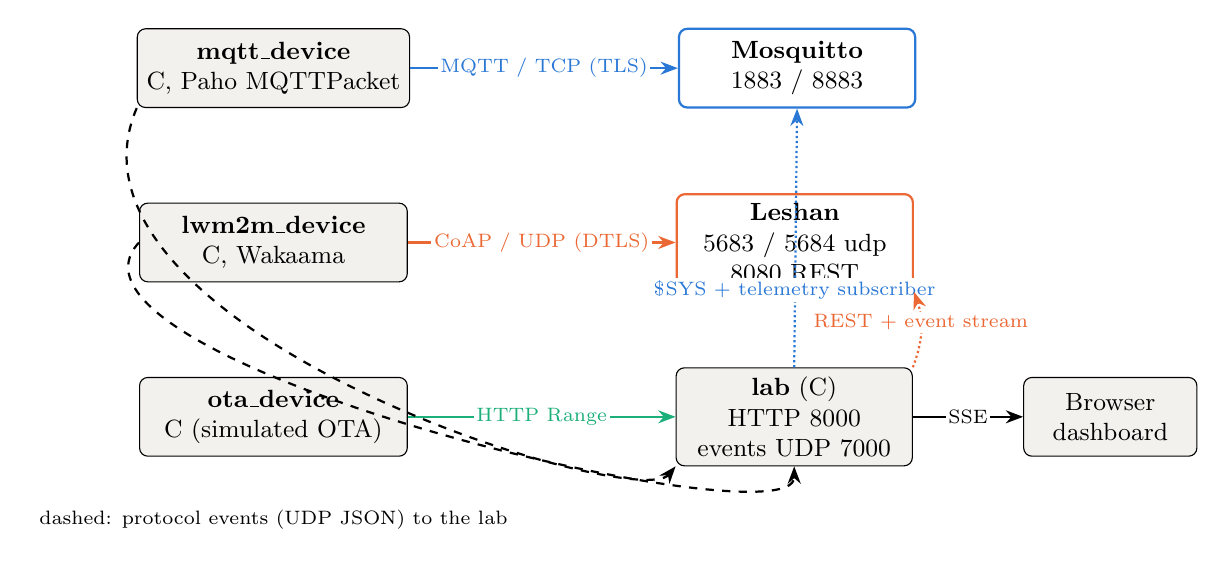
\begin{tikzpicture}[
  node distance=8mm and 10mm,
  box/.style={draw, rounded corners=3pt, fill=boxfill, align=center,
              minimum height=10mm, font=\small},
  srv/.style={box, fill=white, line width=0.8pt},
  arr/.style={-{Stealth[length=2.2mm]}, thick},
  lbl/.style={font=\scriptsize, midway, fill=white, inner sep=1pt}]
  \node[box, minimum width=34mm] (mq) {\textbf{mqtt\_device}\\C, Paho MQTTPacket};
  \node[box, minimum width=34mm, below=12mm of mq] (lw) {\textbf{lwm2m\_device}\\C, Wakaama};
  \node[box, minimum width=34mm, below=12mm of lw] (ot) {\textbf{ota\_device}\\C (simulated OTA)};
  \node[srv, right=34mm of mq, minimum width=30mm, draw=mqtt] (mosq) {\textbf{Mosquitto}\\1883 / 8883};
  \node[srv, right=34mm of lw, minimum width=30mm, draw=lwm2m] (lesh) {\textbf{Leshan}\\5683 / 5684 udp\\8080 REST};
  \node[box, right=34mm of ot, minimum width=30mm] (lab) {\textbf{lab} (C)\\HTTP 8000\\events UDP 7000};
  \node[box, right=14mm of lab, minimum width=22mm] (br) {Browser\\dashboard};

  \draw[arr, mqtt] (mq) -- node[lbl]{MQTT / TCP (TLS)} (mosq);
  \draw[arr, lwm2m] (lw) -- node[lbl]{CoAP / UDP (DTLS)} (lesh);
  \draw[arr, ota] (ot) -- node[lbl]{HTTP Range} (lab);
  \draw[arr, dashed] (mq.south west) .. controls +(-1.2,-2.8) and +(-0.5,-0.6) .. (lab.south west);
  \draw[arr, dashed] (lw.west) .. controls +(-1.4,-1.5) and +(0,-1) .. (lab.south);
  \node[font=\scriptsize, align=center] at ($(ot.south)+(0,-8mm)$) {dashed: protocol events (UDP JSON) to the lab};
  \draw[arr] (lab) -- node[lbl]{SSE} (br);
  \draw[arr, mqtt, densely dotted] (lab.north) -- node[lbl, pos=0.3]{\$SYS + telemetry subscriber} (mosq.south);
  \draw[arr, lwm2m, densely dotted] (lab.north east) to[bend right=20] node[lbl, pos=0.6]{REST + event stream} (lesh.south east);
\end{tikzpicture}
\caption{Processes and connections. Each device is a separate program; the lab
starts them, receives their events, watches both servers and serves the dashboard.}
\end{figure}

Four kinds of programs run on the PC:
\begin{enumerate}
  \item \textbf{Simulated devices} (\code{mqtt\_device}, \code{lwm2m\_device},
        \code{ota\_device}) -- C programs, one per protocol. Each can run on
        its own from a terminal or be started by the lab.
  \item \textbf{Real servers} -- Mosquitto (MQTT broker) and Leshan (LwM2M
        server), started by scripts or Docker.
  \item \textbf{The lab} -- a C web server that hosts the dashboard, relays
        device events to the browser, starts/stops devices, proxies Leshan's
        REST API, keeps its own view of both servers, serves OTA images and
        stores benchmark results.
  \item \textbf{The browser dashboard} -- HTML, CSS and plain JavaScript with
        no external libraries (works offline); visualisation only.
\end{enumerate}

\subsection{Why this split}
\begin{itemize}
  \item Devices stay small and portable: no web or UI code inside them, only
        a one-way event side channel that can be turned off (\code{--lab off}).
  \item Devices can be used without the dashboard, exactly like firmware on a
        bench with a serial console.
  \item The server-side truth is observed independently of the device: the
        lab subscribes to the broker and follows Leshan's event stream, so the
        dashboard can show what the \emph{server} received next to what the
        \emph{device} believes it sent.
\end{itemize}

%======================================================================
\section{Device software architecture}

\begin{figure}[h]
\centering
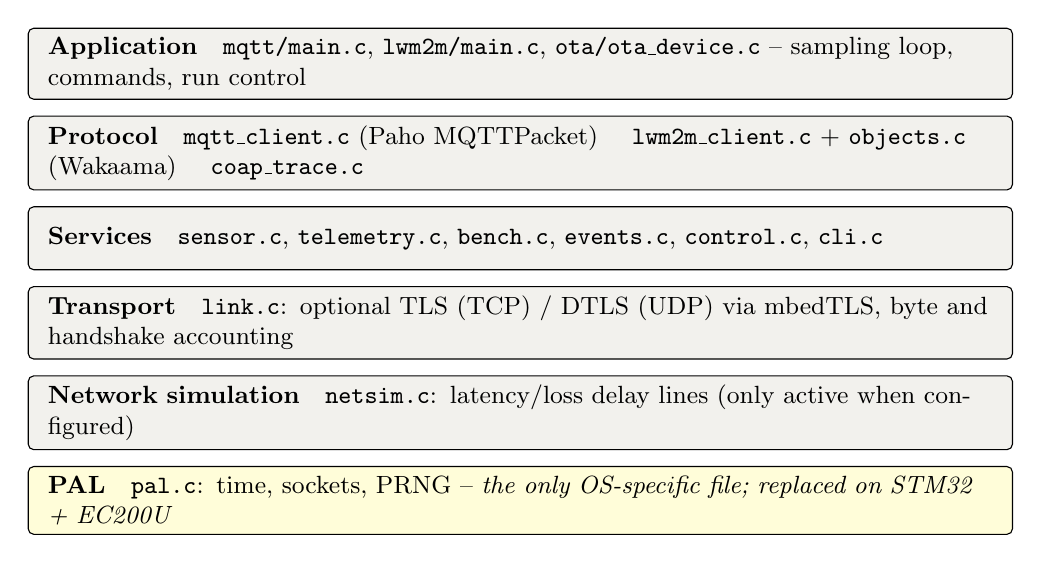
\begin{tikzpicture}[
  lay/.style={draw, rounded corners=2pt, fill=boxfill, minimum width=125mm,
              minimum height=8mm, align=left, font=\small, text width=120mm},
  arr/.style={-{Stealth[length=2mm]}, thick}]
  \node[lay] (app) {\textbf{Application}\quad \code{mqtt/main.c}, \code{lwm2m/main.c}, \code{ota/ota\_device.c} -- sampling loop, commands, run control};
  \node[lay, below=2mm of app] (proto) {\textbf{Protocol}\quad \code{mqtt\_client.c} (Paho MQTTPacket) \quad \code{lwm2m\_client.c} + \code{objects.c} (Wakaama) \quad \code{coap\_trace.c}};
  \node[lay, below=2mm of proto] (svc) {\textbf{Services}\quad \code{sensor.c}, \code{telemetry.c}, \code{bench.c}, \code{events.c}, \code{control.c}, \code{cli.c}};
  \node[lay, below=2mm of svc] (link) {\textbf{Transport}\quad \code{link.c}: optional TLS (TCP) / DTLS (UDP) via mbedTLS, byte and handshake accounting};
  \node[lay, below=2mm of link] (sim) {\textbf{Network simulation}\quad \code{netsim.c}: latency/loss delay lines (only active when configured)};
  \node[lay, below=2mm of sim, fill=yellow!15] (pal) {\textbf{PAL}\quad \code{pal.c}: time, sockets, PRNG -- \emph{the only OS-specific file; replaced on STM32 + EC200U}};
\end{tikzpicture}
\caption{Layers inside every simulated device. Each layer only calls the one below.}
\end{figure}

\subsection{Platform abstraction layer (\code{pal.c})}
All operating-system access lives here: monotonic and wall-clock time, sleep,
sockets (connect, send, receive with timeout, close, local UDP bind, TCP
listen/accept) and a deterministic xorshift PRNG. Windows (Winsock) and POSIX
are both implemented. The socket API is deliberately the same shape as a
cellular modem's AT socket service, which is what makes the later port cheap
(Section~\ref{sec:port}).

\subsection{Transport (\code{link.c})}
A \code{link\_t} is a connection to one server:
\begin{itemize}
  \item TCP or UDP; with security enabled, TLS over TCP or DTLS over UDP using
        mbedTLS 3.6.
  \item Counts \textbf{wire bytes} (what crosses the socket, including TLS/DTLS
        record overhead), packets, TCP connect time, handshake time and
        handshake bytes in each direction.
  \item TLS: verifies the broker certificate against a CA file and expected
        name; TLS~1.3 by default, \code{--tls12} caps at 1.2.
  \item DTLS: pre-shared key, cipher suites \code{TLS\_PSK\_WITH\_AES\_128\_CCM\_8}
        and \code{TLS\_PSK\_WITH\_AES\_128\_CBC\_SHA256}, RFC~6347 retransmission
        timers.
\end{itemize}
The protocol code only calls \code{link\_send} / \code{link\_recv}; it does not
know whether the link is encrypted or impaired.

\subsection{Simulated sensor (\code{sensor.c})}
\code{SensorData\_t} holds temperature (20--35\,\textdegree C), humidity
(30--90\,\%), pressure (990--1030\,hPa) and battery (0--100\,\%). Each channel is
a mean-reverting random walk (discrete Ornstein--Uhlenbeck process) clamped to
its range, so values drift gradually. Humidity is weakly anti-correlated with
temperature; the battery drains slowly and is ``swapped'' at 0\,\%. A seed
(\code{--seed}) makes the sequence fully reproducible.

\subsection{Telemetry payload (\code{telemetry.c})}
Both protocols carry the same JSON document:
\begin{lstlisting}
{"dev":"mqtt-dev-1","seq":12,"ts":1730000000000,"temperature":27.41,
 "humidity":62.10,"pressure":1012.30,"battery":87}
\end{lstlisting}
For payload-size experiments a \code{"pad"} field is added so the document is
exactly the requested number of bytes.

\subsection{Event reporting and control (\code{events.c}, \code{control.c})}
Every protocol message is reported twice: as a human-readable console line and
as a JSON datagram to the lab (UDP 127.0.0.1:7000). A JSON event contains the
protocol, direction, message type, lengths, QoS, latency, security label, a
short detail text, the payload (truncated) and the raw bytes as hex. Devices
also listen on a local UDP control port (7101 MQTT, 7102 LwM2M, 7103 OTA) for
text commands such as \code{stop}, \code{notify}, \code{deregister},
\code{interrupt}. Both channels are lab plumbing, not part of either protocol.

%======================================================================
\section{MQTT device}

\subsection{Approach}
Eclipse Paho's \textbf{MQTTPacket} library only serialises and parses MQTT
packets; it does no I/O. The playground owns the socket
(\code{mqtt\_client.c}), so it can time each exchange precisely and count
every byte. This is also the usual structure on a microcontroller.

\subsection{Session flow}
\begin{lstlisting}
DEVICE                                   BROKER
  | TCP connect                             |
  | [TLS handshake]          (--secure)     |
  | CONNECT client_id keepalive clean ----> |
  | <---------------------- CONNACK rc=0    |
  | SUBSCRIBE playground/<id>/cmd QoS1 ---> |
  | <--------------------------- SUBACK     |
  | PUBLISH playground/<id>/telemetry ----> |  every --interval
  |      ... acknowledgement per QoS ...    |
  | PINGREQ / PINGRESP  (keep-alive)        |
  | DISCONNECT ---------------------------> |
\end{lstlisting}
QoS 0, 1 and 2 are supported in both directions. The command topic lets the
broker deliver commands (\code{interval=}, \code{qos=}, \code{publish},
\code{pause}, \code{resume}, \code{stop}) to the device, which demonstrates the
subscribe path.

\subsection{QoS flows and latency}
\begin{center}
\begin{tabular}{@{}lll@{}}
\toprule
QoS & Packets & Latency definition \\
\midrule
0 & PUBLISH & PUBLISH $\rightarrow$ PINGRESP of a trailing PINGREQ \\
1 & PUBLISH, PUBACK & PUBLISH $\rightarrow$ PUBACK \\
2 & PUBLISH, PUBREC, PUBREL, PUBCOMP & PUBLISH $\rightarrow$ PUBCOMP \\
\bottomrule
\end{tabular}
\end{center}
QoS~0 has no acknowledgement, so ``broker receipt'' is not directly
observable. MQTT runs over a single ordered TCP stream that the broker reads in
order; a PINGREQ sent immediately after the PUBLISH can only be answered after
the PUBLISH has been read. Its PINGRESP therefore proves receipt. The probe
costs 4 bytes per message, which appear in the byte counts;
\code{--no-probe} disables it and the latency is then reported as not measured.

%======================================================================
\section{LwM2M device}

\subsection{Approach}
Eclipse \textbf{Wakaama} (pinned to the 2026-05-26 snapshot, commit
\code{94ff56f}) implements the LwM2M state machine, CoAP and the data formats
(TLV, SenML JSON/CBOR). The playground supplies Wakaama's platform and
transport callbacks (\code{lwm2m\_connect\_server}, \code{lwm2m\_buffer\_send},
\code{lwm2m\_close\_connection}, memory and time functions) on top of
\code{link\_t}, and implements the objects.

\subsection{Objects}
\begin{longtable}{@{}lp{6.2cm}cp{4.3cm}@{}}
\toprule
Path & Meaning & Ops & Notes \\
\midrule
\endhead
\code{/0/0} & Security: server URI, mode (PSK/NoSec), keys & -- & never readable by a server \\
\code{/1/0/1} & Server: lifetime & RW & default 300\,s \\
\code{/1/0/8} & Server: registration update trigger & E & sends UPDATE \\
\code{/3/0/0..3} & Device: manufacturer, model, serial, FW version & R & \\
\code{/3/0/4} & Device: reboot & E & simulated \\
\code{/3/0/9} & Device: \textbf{battery level} (\%) & R & battery lives here \\
\code{/3/0/11} & Device: error code & R & multi-instance \\
\code{/3/0/13..15} & Device: current time, UTC offset, timezone & RW & \\
\code{/19/0/0} & BinaryAppDataContainer: data & R & telemetry JSON, sized by \code{--payload} \\
\code{/3303/0/5700} & Temperature value (Cel) & R & also min/max, range, units \\
\code{/3303/0/5605} & Temperature: reset min/max & E & \\
\code{/3303/0/5750} & Temperature: application type & RW & good Write target \\
\code{/3304/0/5700} & Humidity (\%RH) & R & same resource set \\
\code{/3315/0/5700} & Barometer (hPa) & R & same resource set \\
\bottomrule
\end{longtable}
OMA's core object set has no stand-alone battery object; battery level is
resource 9 of the Device object (\code{/3/0/9}). \code{/3/0/13} is Current Time.

All objects share one \textbf{table-driven engine} (\code{objects.c}): an object
is a resource table (id and allowed operations) plus get/set/execute
callbacks; read, write, execute and discover are implemented once. This keeps
the code small, which also suits a microcontroller.

\subsection{Transactions}
\begin{lstlisting}
REGISTER    D -- CON POST /rd?ep=..&lt=300&lwm2m=1.1&b=U  (link-format) --> S
            D <-------------------------- ACK 2.01 Created, Location /rd/<id>
READ        S -- CON GET  /3/0/9 ----------> D -- ACK 2.05 + value -------> S
WRITE       S -- CON PUT  /3303/0/5750 ----> D -- ACK 2.04 ---------------> S
EXECUTE     S -- CON POST /3303/0/5605 ----> D -- ACK 2.04 ---------------> S
OBSERVE     S -- CON GET  /3303/0/5700 Obs:0 -> D -- ACK 2.05 Obs:n + value -> S
NOTIFY      D -- CON 2.05 Obs:n+1 + value (same token) -----------------> S
            D <-------------------------------------------- empty ACK -- S
DEREGISTER  D -- CON DELETE /rd/<id> ----------------------------------> S
            D <--------------------------------------------- ACK 2.02 -- S
\end{lstlisting}

\subsection{CoAP tracing}
\code{coap\_trace.c} decodes every datagram Wakaama sends or receives (type,
code, Message ID, token, Uri-Path/Query, Observe, Content-Format) and names it
the way the LwM2M specification does (REGISTER, OBSERVE, NOTIFY, READ
RESPONSE, ...). A small table of outstanding confirmable requests per direction
matches each ACK to its request by Message ID, which yields the latency and
detects retransmissions (same Message ID sent again).

\subsection{Confirmable notifications}
Wakaama sends Observe notifications as \textbf{NON} (non-confirmable). Nothing
acknowledges them, so neither delivery nor latency can be measured and a lost
notification is silently gone. RFC~7641 allows either type, so the playground
flips each outgoing notification to \textbf{CON} and takes over its
reliability using RFC~7252 timing:
\begin{itemize}
  \item initial timeout \code{ACK\_TIMEOUT} $\times$ random$[1, 1.5]$ (2--3\,s by default);
  \item retransmit the same message (same Message ID), doubling the timeout;
  \item give up after \code{MAX\_RETRANSMIT} = 4 retransmissions
        (62--93\,s after the first transmission).
\end{itemize}
Latency is CON $\rightarrow$ ACK measured from the \emph{first} transmission.
\code{--notify-non} restores the stock behaviour, in which case latency is
honestly reported as not measured.

A notification can end in RST, which counts as a failure: Leshan rejects a
retransmitted notification once it already has a newer one, and notifications
in flight are rejected when a second OBSERVE replaces the observation (new
token).

%======================================================================
\section{The lab server and dashboard}

\subsection{Lab server (C)}
\code{lab} is a small multi-threaded HTTP/1.1 server bound to 127.0.0.1:
\begin{longtable}{@{}p{4.5cm}p{10cm}@{}}
\toprule
Route & Purpose \\
\midrule
\endhead
\code{/}, static files & dashboard (\code{dashboard/www}) \\
\code{/api/events} & Server-Sent Events: every device/lab/server event, with a 3000-event replay buffer for new browser tabs \\
\code{/api/state} & snapshot of broker, Leshan and device state \\
\code{/api/device/start|stop|cmd} & start a device with validated parameters, stop it gracefully (DISCONNECT / De-register) or send a control command \\
\code{/api/mqtt/publish} & publish via the lab's broker connection (device commands) \\
\code{/api/runs}, \code{/results/*.csv} & benchmark summaries and per-message CSV files \\
\code{/leshan/...} & reverse proxy to Leshan's REST API and event stream \\
\code{/ota/manifest}, \code{/ota/<image>} & SIMULATED OTA images with HTTP Range support \\
\code{/docs/*} & the Markdown documentation \\
\bottomrule
\end{longtable}

Background threads:
\begin{itemize}
  \item \textbf{Event receiver}: UDP 7000; stores the latest state per device,
        appends run summaries to \code{results/runs.jsonl}, broadcasts
        everything to the browsers.
  \item \textbf{MQTT monitor}: its own MQTT connection; subscribes to
        \code{\$SYS/broker/...} statistics and \code{playground/+/telemetry}, so
        the dashboard shows what the broker actually delivered.
  \item \textbf{Leshan monitor}: polls \code{/api/clients} and follows
        Leshan's \code{/api/event} stream (registrations, notifications) using
        HTTP/1.0 so responses are never chunked.
  \item \textbf{Reaper}: notices when device processes exit.
\end{itemize}
Device parameters coming from the browser are whitelisted per device and
restricted to simple tokens before a process is spawned (no shell is
involved). When an LwM2M device is started with security on, the lab first
registers its PSK in Leshan; with security off it removes any stale PSK.

\subsection{Dashboard}
Plain HTML/CSS/JavaScript, no external libraries. Tabs:
\begin{itemize}
  \item \textbf{MQTT}: QoS 0/1/2 selector, interval, count, payload size,
        security toggle, network profile; START/STOP/RESET; animated sequence
        diagram (DEVICE $\leftrightarrow$ BROKER); the selected QoS's message
        flow; broker panel (from \$SYS and the lab subscriber); device panel;
        live latency chart.
  \item \textbf{LwM2M}: same controls plus CON/NON; device operations
        (Register, Deregister, Notify) and server operations through Leshan
        (Read, Write, Observe, Cancel observe, Execute) on a selectable
        resource table; sequence diagram (DEVICE $\leftrightarrow$ SERVER);
        Leshan panel; auto-OBSERVE after registration.
  \item \textbf{MQTT vs LwM2M}: side-by-side table of the latest run of each
        (``Not measured'' when absent), one-click experiments, six charts and a
        table of all runs with CSV links.
  \item \textbf{OTA}: image and chunk size, network profile, START / INTERRUPT /
        RESET, animated step list, progress bar and statistics, size-vs-time chart.
  \item \textbf{Event log and message inspector} (all tabs): click any event to
        see protocol, direction, type, lengths, security, timestamp, latency,
        CoAP header fields and a hex dump of the raw bytes.
\end{itemize}
Charts are hand-written SVG with a colour-vision-checked palette (MQTT blue,
LwM2M orange, OTA aqua), a legend and direct labels, and hover tooltips.
Redraws are coalesced (at most about eight per second) so bursts of events stay
cheap, and the experiment runner advances on the lab's ``device exited''
event, which is not slowed by browsers' background-tab timer throttling.

%======================================================================
\section{End-to-end workflow}

\subsection{Build}
\begin{lstlisting}
cmake -S . -B build
cmake --build build
ctest --test-dir build
\end{lstlisting}
The first configure fetches mbedTLS 3.6.7, Paho Embedded-C 1.1.0 and Wakaama
(pinned commit) with CMake FetchContent. Outputs: \code{mqtt\_device},
\code{lwm2m\_device}, \code{ota\_device}, \code{lab}, unit tests, and the sample
images \code{build/ota/firmware\_v1.bin} (64\,KiB) and \code{firmware\_v2.bin}
(256\,KiB).

\subsection{Start the servers}
\begin{center}
\begin{tabularx}{\textwidth}{@{}lX@{}}
\toprule
Option & Commands \\
\midrule
Docker & \code{docker compose up} (official \code{eclipse-mosquitto:2} image; Leshan built from \code{servers/leshan/Dockerfile}) \\
Windows, no Docker & \code{scripts\textbackslash get-servers.ps1} once (portable Mosquitto, Java, Leshan in \code{servers\textbackslash.local}), then \code{start-mosquitto.ps1} and \code{start-leshan.ps1} \\
Linux/macOS/WSL & \code{scripts/get-servers.sh} once, then \code{start-mosquitto.sh} and \code{start-leshan.sh} \\
\bottomrule
\end{tabularx}
\end{center}
On the development PC, Windows (Hyper-V/WinNAT) reserves TCP ports 1827--1926,
which includes 1883. Either reserve 1883 with
\code{netsh int ipv4 add excludedportrange} (admin) or use other ports, e.g.
\code{start-mosquitto.ps1 -Port 21883 -TlsPort 28883} and
\code{lab --mqtt-port 21883 --mqtts-port 28883}.

\subsection{Run}
\begin{enumerate}
  \item Start \code{lab} and open \url{http://127.0.0.1:8000}; both server
        indicators must read ONLINE.
  \item MQTT tab $\rightarrow$ START: watch CONNECT $\rightarrow$ CONNACK
        $\rightarrow$ SUBSCRIBE $\rightarrow$ SUBACK $\rightarrow$ PUBLISH
        $\rightarrow$ PUBACK.
  \item LwM2M tab $\rightarrow$ START: REGISTER $\rightarrow$ 2.01, automatic
        OBSERVE, then NOTIFY $\rightarrow$ ACK every interval; try Read, Write,
        Execute.
  \item MQTT vs LwM2M $\rightarrow$ ``Benchmark: 100 + 100'', then the loss,
        latency, payload and security experiments.
  \item OTA tab $\rightarrow$ START OTA, then INTERRUPT on a poor network.
\end{enumerate}

\subsection{Data flow of one MQTT message}
\begin{enumerate}
  \item The device samples the sensor, builds the JSON payload, serialises a
        PUBLISH with Paho, timestamps it and hands it to \code{link\_send}.
  \item \code{netsim} (if active) holds the packet; TLS encrypts it; the PAL
        writes it to the socket. Wire bytes are counted.
  \item Mosquitto delivers it to the lab's subscriber and answers PUBACK.
  \item The device reads the PUBACK, computes PUBLISH $\rightarrow$ PUBACK
        latency and records one benchmark row.
  \item For both packets the device emits a console line and a JSON event to
        the lab, which pushes them to the browser; the broker panel updates
        from the lab's subscriber and \$SYS counters.
\end{enumerate}

%======================================================================
\section{Measurement methodology}

\subsection{What is recorded}
Per message (\code{results/<run>.csv}):
\code{seq, timestamp\_ms, latency\_ms, payload\_bytes, bytes\_sent,
bytes\_received, success, retries}. Bytes are \emph{wire} bytes of that
message's whole exchange (including TLS/DTLS overhead, PUBREL, the QoS~0 probe
and CoAP retransmissions). Per run (\code{results/runs.jsonl}): configuration,
counts, success rate, min/avg/median/P95/P99/max latency, average bytes,
connection time, handshake time and bytes.

\subsection{Latency}
\begin{center}
\begin{tabular}{@{}ll@{}}
\toprule
Protocol & From $\rightarrow$ to \\
\midrule
MQTT QoS 0 & PUBLISH $\rightarrow$ PINGRESP of the trailing PINGREQ \\
MQTT QoS 1 & PUBLISH $\rightarrow$ PUBACK \\
MQTT QoS 2 & PUBLISH $\rightarrow$ PUBCOMP \\
LwM2M & CON $\rightarrow$ ACK of each notification, from its first transmission \\
\bottomrule
\end{tabular}
\end{center}
All timestamps are taken \emph{before} the message is handed to the network
layer, so simulated delay is always inside the measured interval.

\subsection{Statistics}
Statistics are computed over successful messages only. Percentiles use the
\textbf{nearest-rank} method: the $p$-th percentile of $n$ sorted values is the
$\lceil p\,n/100\rceil$-th value. With 100 messages P99 is the 99th value; with
20 messages P95 and P99 both equal the maximum, so small runs say little about
the tail. A failed message counts against the success rate and never gets a
latency. A value that was not measured is serialised as \code{null} and shown
as ``Not measured''.

\subsection{Connection cost}
\emph{Time to ready} = socket setup + TLS/DTLS handshake + protocol session
(CONNECT/CONNACK for MQTT, REGISTER/2.01 for LwM2M). Handshake time and
handshake bytes are reported separately.

%======================================================================
\section{Network simulation}

\subsection{Built-in model (all platforms)}
\code{netsim} sits between the protocol and the socket, below TLS/DTLS, and
implements a \textbf{delay line in each direction}:
\begin{itemize}
  \item \textbf{Latency}: every outgoing packet waits for the one-way latency
        before reaching the socket; every incoming packet waits for it before
        the device sees it. A request/response therefore costs
        $2L$ plus the real round trip, a QoS~2 exchange $4L$, a DTLS~1.2 PSK
        handshake (three round trips) $6L$, independent of how many packets
        are in flight; a server-initiated request arrives $L$ late.
  \item \textbf{Loss, UDP} (LwM2M): datagrams are really dropped in either
        direction; CoAP and DTLS must retransmit.
  \item \textbf{Loss, TCP} (MQTT): dropping bytes would corrupt the stream, so
        a lost segment is delivered one retransmission timeout later instead
        (\code{--rto}, default 200\,ms, doubling for consecutive losses), with
        order preserved -- which is what the kernel's TCP would do.
\end{itemize}
Profiles: Excellent (0\,ms, 0\,\%), Good (50\,ms, 1\,\%), Poor (250\,ms, 5\,\%),
Very Poor (1000\,ms, 10\,\%), or Custom. It is a teaching model: no jitter,
bandwidth limit or reordering.

\subsection{Kernel model (Linux/WSL)}
\code{scripts/netem.sh} applies \code{tc netem} delay and loss to the server
ports on the loopback interface (requires root). The dashboard's own network
controls should then be set to 0\,ms / 0\,\%.

%======================================================================
\section{Security experiments}
\begin{center}
\begin{tabular}{@{}lll@{}}
\toprule
 & Security off & Security on \\
\midrule
MQTT & TCP, port 1883 & TLS 1.3 (or 1.2), port 8883, server certificate verified \\
LwM2M & CoAP/UDP, port 5683 & DTLS 1.2 PSK, port 5684 \\
\bottomrule
\end{tabular}
\end{center}
The broker certificate is signed by a lab CA committed in
\code{servers/mosquitto/certs} (lab use only; \code{gen-certs.sh} regenerates
it). For DTLS the PSK must also be known to Leshan; the dashboard registers it
through Leshan's REST API before a secure run and removes it before a plain
run, because Leshan rejects a plain-CoAP registration with \textbf{4.03
Forbidden} for an endpoint that has a PSK. Unsupported modes (client
certificates, RPK, OSCORE, bootstrap) are not offered in the UI.

%======================================================================
\section{Simulated OTA}
Clearly labelled as a \textbf{simulation}: it does not model STM32 flash,
banks, bootloaders, signing or rollback.
\begin{lstlisting}
Server  -- GET /ota/manifest?image=X --> {version, size, sha256}  (firmware available)
Device  -- GET /ota/X  Range: bytes=a-b --> one chunk per request  (download)
Device  -- write chunk --> results/ota_storage/slot_b.bin          (storage)
Device  -- SHA-256(slot B) == manifest.sha256 ?                    (verify)
Device  -- write version --> active_version.txt                    (activate)
\end{lstlisting}
The download uses the same link and network simulation as the protocols, so
latency and loss slow it down in the same way. Chunked range requests (default
1\,KiB) mimic a modem-attached MCU fetching an image block by block; a failed
chunk is retried up to three times. Interrupt aborts the download (the running
version is unchanged); reset wipes slot B and returns to v1.0.0. Reported:
firmware size, download, verify and total time, wire bytes, chunks, retries,
completion or failure reason. Images are deterministic pseudo-random data with
a small header; besides \code{firmware\_v1/v2.bin} the lab generates
\code{fw\_<N>k.bin} on demand for size sweeps.

%======================================================================
\section{Verification approach}
\begin{itemize}
  \item \textbf{Unit tests} (\code{ctest}, 5 suites): sensor range,
        smoothness and reproducibility; nearest-rank percentiles and
        ``not measured'' serialisation; exact payload padding; the network
        model (per-packet delay, UDP loss rate, TCP never drops); CoAP decoding,
        LwM2M naming, retransmission detection and latency from first send.
  \item \textbf{Real-server tests}: every MQTT QoS level, TLS~1.3 with
        verification, every LwM2M operation (Register, Read, Write, Execute,
        Observe, Cancel, Notify, Update, Deregister), DTLS-PSK, OTA with and
        without impairment and with interrupt -- against Mosquitto 2.1.2 and
        Leshan 2.0.0-M18.
  \item \textbf{Physics checks of the network model}: at 200\,ms one-way
        latency QoS~1 measured $\approx$ 415\,ms (one round trip), QoS~2
        $\approx$ 825\,ms (two), TLS~1.3 handshake $\approx 2L$, DTLS~1.2 PSK
        handshake $\approx 6L$.
  \item \textbf{Cross-checks}: the device's own counts compared with the
        server-side view (lab MQTT subscriber, Leshan's event stream), e.g. 10
        notifications ACKed on the device and 10 NOTIFICATION events from
        Leshan.
  \item \textbf{Browser tests}: all tabs exercised in Chrome, including the
        experiment runner.
  \item \textbf{Linux build}: clean build and passing tests under WSL
        (GCC 15), plus a runtime smoke test of the lab and devices.
\end{itemize}

%======================================================================
\section{Problems found and how they were solved}
\begin{longtable}{@{}p{4.6cm}p{10cm}@{}}
\toprule
Problem & Resolution \\
\midrule
\endhead
Port 1883 refused on Windows & Port range reserved by Hyper-V/WinNAT. All ports made configurable; documented the \code{netsh} reservation and alternate ports. \\
Wakaama notifications are NON & Converted to CON with RFC~7252 retransmission in the transport glue; NON kept as an option. \\
LwM2M REGISTER got 4.03 & Stale PSK in Leshan after a DTLS run; the lab now removes it for plain runs and the device explains the error. \\
In-flight notifications counted as failed at the end of a run & Device stops producing when the count is sent or in flight, then waits for each to be ACKed or exhausted. \\
LwM2M ``time to registered'' inflated by the main-loop tick & Registration is checked immediately after each received packet. \\
LwM2M latency missed the outbound delay & Timestamps moved to before \code{link\_send}, consistent with MQTT. \\
First network model charged latency only on direction changes (back-to-back packets skipped the delay) & Replaced with per-packet delay lines in both directions; verified against round-trip counts. \\
Dashboard slowed under heavy event bursts and background-tab throttling & Coalesced redraws, bounded series, event-driven experiment runner. \\
Mosquitto 2.1 deprecations / inline comments & Configuration cleaned (no \code{per\_listener\_settings}, comments on their own lines). \\
\bottomrule
\end{longtable}

%======================================================================
\section{Measured results (development PC)}
Windows 11, loopback, Mosquitto 2.1.2, Leshan 2.0.0-M18, MQTT QoS~1, LwM2M CON
notifications, natural payload, interval 0.2\,s. These are measurements from one
machine, not general claims; loopback numbers show protocol overhead, not radio
behaviour.

\begin{center}
\begin{tabular}{@{}lrrrr@{}}
\toprule
 & \multicolumn{2}{c}{MQTT} & \multicolumn{2}{c}{LwM2M} \\
\cmidrule(lr){2-3}\cmidrule(lr){4-5}
Run & median & P95 & median & P95 \\
\midrule
Benchmark, 100 messages, no impairment & 0.38\,ms & 0.71\,ms & 1.17\,ms & 2.74\,ms \\
Loss 1\,\% (50 messages) & 0.37\,ms & 0.53\,ms & 1.02\,ms & 1.80\,ms \\
Loss 2\,\% & 0.37\,ms & 0.54\,ms & 1.07\,ms & 1.79\,ms \\
Loss 5\,\% & 0.37\,ms & 208\,ms & 1.07\,ms & 2769\,ms \\
Loss 10\,\% & 0.43\,ms & 213\,ms & 0.96\,ms & 6181\,ms \\
\bottomrule
\end{tabular}
\end{center}
All runs above delivered 100\,\% of messages.

\begin{center}
\begin{tabular}{@{}lrrrr@{}}
\toprule
 & \multicolumn{2}{c}{MQTT} & \multicolumn{2}{c}{LwM2M} \\
\cmidrule(lr){2-3}\cmidrule(lr){4-5}
Security & off & TLS 1.3 & off & DTLS 1.2 \\
\midrule
Time to ready & 0.76\,ms & 12.7\,ms & 2.6\,ms & 25.3\,ms \\
Wire bytes per message & 158.7 & 207.0 & 36.8 & 94.8 \\
Handshake bytes & -- & 2812 & -- & 601 \\
\bottomrule
\end{tabular}
\end{center}

\subsection*{Interpretation}
\begin{itemize}
  \item With no impairment both protocols are sub-millisecond to a few
        milliseconds on loopback; LwM2M's slightly higher latency includes the
        CoAP exchange through Wakaama and Leshan.
  \item LwM2M carries far fewer bytes per message here (one resource value,
        compact SenML/CBOR, 4-byte CoAP header) than MQTT carrying the full
        JSON document over TCP.
  \item Under loss both still deliver everything, but recover very
        differently: TCP's 200\,ms retransmission timer bounds MQTT's tail
        around 200\,ms, while CoAP's 2--3\,s ACK timeout with exponential
        backoff pushes LwM2M's P95 to seconds.
  \item Security costs a handshake (TLS~1.3: 1 round trip, 2.8\,KB with the
        certificate; DTLS~1.2 PSK: 3 round trips, 0.6\,KB) and per-record
        overhead on every message.
\end{itemize}

%======================================================================
\section{Known limitations}
\begin{itemize}
  \item The built-in network model has no jitter, reordering or bandwidth
        limit; use \code{tc netem} for packet-accurate impairment.
  \item LwM2M notifications are confirmable by design choice; stock Wakaama
        behaviour is available with \code{--notify-non}.
  \item OTA is a simulation; LwM2M Object~5 firmware update is not implemented.
  \item No bootstrap server, queue mode, client certificates, RPK or OSCORE.
  \item Lab TLS certificates and the default DTLS key are for the lab only.
  \item Not exercised on the development PC: Docker Compose (Docker not
        installed) and \code{netem.sh} (requires root in WSL).
\end{itemize}

%======================================================================
\section{Porting to STM32 + EC200U}\label{sec:port}
Only \code{pal.c} touches the operating system. The rest is portable C:
\begin{center}
\begin{tabularx}{\textwidth}{@{}lX@{}}
\toprule
PC (\code{pal.c}) & STM32 + EC200U \\
\midrule
\code{pal\_now\_us}, \code{pal\_sleep\_ms} & SysTick or a timer; HAL/RTOS delay \\
\code{pal\_sock\_connect} & \code{AT+QIOPEN=1,<id>,"TCP"|"UDP",host,port} $\rightarrow$ \code{+QIOPEN: <id>,0} \\
\code{pal\_sock\_send} & \code{AT+QISEND=<id>,<len>}, data, \code{SEND OK} \\
\code{pal\_sock\_recv} & wait for \code{+QIURC: "recv",<id>}, then \code{AT+QIRD} \\
\code{pal\_sock\_close} & \code{AT+QICLOSE=<id>} \\
entropy for mbedTLS & STM32 RNG peripheral \\
\bottomrule
\end{tabularx}
\end{center}
Unchanged: \code{mqtt\_client.c}, \code{lwm2m\_client.c}, \code{objects.c},
\code{sensor.c} (or a real driver), \code{telemetry.c}, \code{bench.c},
\code{link.c} with a bare-metal mbedTLS configuration. Lab-only parts
(\code{netsim.c}, \code{events.c}, \code{control.c}) are compiled out or
redirected to a debug UART. Points to plan: an interrupt/DMA-driven UART ring
buffer with an AT parser that handles unsolicited result codes; whether TLS
runs on the MCU (full visibility) or in the modem (\code{AT+QSSLOPEN}, less
MCU memory); trimming buffers; real time for certificate checks; LwM2M queue
mode for PSM/eDRX.

%======================================================================
\appendix
\section{Repository layout}
\begin{lstlisting}
CMakeLists.txt, cmake/deps.cmake      build + dependency pinning
device/common/                        pal, link, netsim, sensor, telemetry,
                                      events, control, cli
device/mqtt/                          main.c, mqtt_client.c
device/lwm2m/                         main.c, lwm2m_client.c, objects.c,
                                      coap_trace.c
benchmark/                            bench.c (records, percentiles, CSV)
ota/                                  ota_device.c, make_firmware.c, fw_image.h
dashboard/server/                     lab.c, http.c, monitor.c, proc.c
dashboard/www/                        index.html, style.css, app.js, charts.js
servers/mosquitto/                    configs, lab certificates, gen-certs.sh
servers/leshan/                       Dockerfile
scripts/                              get/start servers (ps1, sh), netem.sh
tests/                                unit tests (ctest)
docs/                                 Markdown guides and this document
docker-compose.yml, README.md
\end{lstlisting}

\section{Command-line reference}
\subsection*{Common device options}
\begin{lstlisting}
--host H  --port N  --id NAME  --interval 10s|500ms  --count N  --payload BYTES
--seed N  --timeout 10s  --secure  --ca FILE  --tls-name NAME  --tls12
--psk-id ID  --psk HEX  --profile excellent|good|poor|very-poor|custom
--latency MS  --loss PERCENT  --rto MS  --lab HOST:PORT|off  --ctl-port N
--results DIR  --run ID
\end{lstlisting}
\subsection*{Device-specific options}
\begin{lstlisting}
mqtt_device   --qos 0|1|2  --no-probe  --keepalive S  --topic PREFIX
              --user U  --pass P
lwm2m_device  --lifetime S  --notify-non  --ack-timeout 2s
ota_device    --image NAME  --chunk BYTES  --action update|reset
lab           --http-port 8000  --events-port 7000  --mqtt-host H
              --mqtt-port 1883  --mqtts-port 8883  --leshan-host H
              --leshan-port 8080  --coap-port 5683  --coaps-port 5684
              --www DIR  --results DIR
\end{lstlisting}

\section{Leshan REST calls used}
\begin{lstlisting}
GET    /api/clients                                   registered clients
GET    /api/clients/<ep>/<path>?timeout=5             READ
PUT    /api/clients/<ep>/<path>?timeout=5             WRITE
       {"id":5750,"kind":"singleResource","value":"kitchen","type":"string"}
POST   /api/clients/<ep>/<path>?timeout=5             EXECUTE
POST   /api/clients/<ep>/<path>/observe               OBSERVE
DELETE /api/clients/<ep>/<path>/observe?active=true   cancel observation
GET    /api/event                                     event stream (SSE)
PUT    /api/security/clients/                         add PSK
       {"endpoint":"lwm2m-dev-1","tls":{"mode":"psk","details":
        {"identity":"lwm2m-dev-1","key":"000102030405060708090a0b0c0d0e0f"}}}
DELETE /api/security/clients/<ep>                     remove PSK
\end{lstlisting}

\end{document}
